% !TeX program = pdflatex
\documentclass[11pt]{beamer}
\usetheme{Madrid}

% ===== Encodage & langue =====
\usepackage[T1]{fontenc}
\usepackage[utf8]{inputenc}
\usepackage[english]{babel}
\usepackage{lmodern}
\usepackage{microtype}
\usepackage[skip=2pt]{caption}
\usepackage{listings}
\usepackage{xcolor}
\usepackage{pdfrender}

% Palette minimale (modifiable)
\definecolor{codebg}{RGB}{245,247,250}
\definecolor{codekw}{RGB}{0,92,197}
\definecolor{codestr}{RGB}{163,21,21}
\definecolor{codecm}{gray}{0.35}
\definecolor{codeid}{RGB}{20,20,140}

\lstdefinestyle{cpp}{
  language=C++,
  basicstyle=\ttfamily\footnotesize,
  keywordstyle=\color{codekw},
  stringstyle=\color{codestr},
  commentstyle=\itshape\color{codecm},
  identifierstyle=\color{codeid},
  backgroundcolor=\color{codebg},
  numbers=left,
  numberstyle=\tiny\color{codecm},
  numbersep=8pt,
  showstringspaces=false,
  breaklines=true,
  tabsize=2,
  columns=fullflexible,
  frame=single
}

% ===== Maths, figures & utilitaires =====
\usepackage{amsmath,amsfonts,amssymb}
\usepackage{graphicx}
\usepackage{booktabs}
\usepackage{siunitx}
\usepackage{adjustbox}
\usepackage{tikz}
\usepackage{pifont}
\graphicspath{{images/}{imagens/}}

% ===== Couleurs & style (accent CEA) =====
\definecolor{ceaGreen}{RGB}{160,0,0}
\definecolor{ceaDarkRed}{RGB}{135,0,0}
\definecolor{ceaGray}{RGB}{230,245,239}
\definecolor{ceaLight}{RGB}{230,245,239}
\definecolor{hlOrange}{RGB}{255,128,0}
\definecolor{hlOrangeBg}{RGB}{255,245,230}
\definecolor{termBg}{RGB}{28,31,36}
\definecolor{termBar}{RGB}{62,67,76}
\definecolor{termText}{RGB}{236,239,244}
\definecolor{hotspotBlue}{RGB}{120,190,255}

\hypersetup{colorlinks=true,linkcolor=black,urlcolor=ceaGreen,citecolor=ceaGreen}

\usetikzlibrary{calc,tikzmark,positioning,arrows.meta,shapes.geometric,fit}
\newcommand{\ScopeLine}[2]{
  \begin{tikzpicture}[remember picture,overlay]
    \draw[green!60!black,line width=1.4pt,line cap=round]
      ($(pic cs:#1)+(0.25em,-0.6ex)$) -- ($(pic cs:#2)+(0.25em,1.2ex)$);
  \end{tikzpicture}%
}

\setbeamercolor{structure}{fg=ceaGreen}
\setbeamercolor{title}{fg=white,bg=ceaGreen}
\setbeamercolor{frametitle}{fg=ceaGray}
\setbeamercolor{block title}{bg=ceaGreen!15,fg=ceaGreen}
\setbeamercolor{block body}{bg=ceaLight}
\setbeamercolor{terminal title}{fg=termText,bg=termBar}
\setbeamercolor{terminal body}{fg=termText,bg=termBg}
\setbeamercolor{profiler title}{fg=white,bg=hlOrange!85!black}
\setbeamercolor{profiler body}{fg=black,bg=hlOrangeBg}
\setbeamercolor{tuner title}{fg=white,bg=ceaGreen}
\setbeamercolor{tuner body}{fg=black,bg=ceaLight}
\setbeamercolor{section foot}{fg=white,bg=ceaGreen}
\setbeamercolor{framenum foot}{fg=white,bg=ceaGreen}
\setbeamertemplate{caption}[numbered]
\setbeamertemplate{navigation symbols}{}
\setbeamertemplate{footline}{
  \leavevmode%
  
\begin{tikzpicture}[x=1pt,y=1pt,baseline]
    \fill[ceaGreen] (0,0) rectangle (\paperwidth,15);
    \node[anchor=west] at (8,7.5) {{\color{white}\bfseries\tiny\secname}};
    \node[anchor=center] at (\dimexpr.975\paperwidth\relax,7.5) {{\color{white}\tiny\insertframenumber}};
  \end{tikzpicture}%
}
\setbeamertemplate{section page}{
  \begin{center}
    \vspace*{\fill}
    {\color{ceaGreen}\bfseries\LARGE\insertsectionhead\par}
    \vspace*{\fill}
  \end{center}
}
\AtBeginSection[]{
  \ifnum\value{section}>1\relax
    \begin{frame}[plain]
      \sectionpage
    \end{frame}
  \fi
}

% ===== Raccourcis utiles =====
\newcommand{\dyablo}{Dyablo}
\newcommand{\cmark}{\ding{51}}
\newcommand{\xmark}{\ding{55}}
\newcommand{\todo}[1]{\textcolor{red}{\textbf{TODO:~#1}}}
\newcommand{\email}{\texttt{jean-francois.david@cea.fr}}

% ===== Listings =====
\lstset{
  basicstyle=\ttfamily\small,
  breaklines=true,
  frame=single,
  columns=fullflexible,
  keywordstyle=\color{codekw},
  language=C++,
  showstringspaces=false,
  morekeywords={Kokkos,View,parallel_for,parallel_reduce,TeamPolicy,RangePolicy}
}

\lstdefinestyle{terminal}{
  basicstyle=\ttfamily\tiny\color{termText},
  backgroundcolor=\color{termBg},
  breaklines=true,
  columns=fullflexible,
  frame=none,
  keepspaces=true,
  keywordstyle=\color{termText},
  commentstyle=\color{termText},
  stringstyle=\color{termText},
  identifierstyle=\color{termText},
  showstringspaces=false,
  aboveskip=0pt,
  belowskip=0pt
}

% ===== Métadonnées =====

\title[APEX @ Dyablo]{APEX on Dyablo\\Profiling and Auto-Tuning Kokkos Kernels}
\author[David, Durocher, Delorme]{Jean-François David \and Arnaud Durocher \and Maxime Delorme}
\date{CEA / CExA\\\today}

\begin{document}

\begin{frame}
  \titlepage
\end{frame}

% =========================================================
\section{1. Context}
% =========================================================

\begin{frame}[t]{Case study: using APEX on Dyablo}
\small
\begin{itemize}\itemsep0.4em
    \item Dyablo is a Kokkos-based AMR hydrodynamics / MHD application targeting CPU and GPU executions.
    \item APEX is a performance measurement and auto-tuning framework that can plug into Kokkos.
    \item In this presentation, \dyablo{} is used as an example to show:
    \begin{itemize}\itemsep0.2em
        \item how APEX profiles a GPU application
        \item how APEX tunes Kokkos internal execution parameters
    \end{itemize}
    \item Integration branch: \href{https://github.com/daxmawal/Dyablo-apex/tree/apex}{\texttt{daxmawal/Dyablo-apex}, branch \texttt{apex}}.
    \item All Dyablo examples in this presentation are run with \texttt{test\_blast\_2D\_block.ini}.
    \item \todo{Use a larger test case than \texttt{test\_blast\_2D\_block.ini}.}
\end{itemize}
\end{frame}

\begin{frame}[t]{Two complementary roles}
\begin{beamerboxesrounded}[upper=profiler title,lower=profiler body,width=\linewidth,shadow=false]{Profiler}
\small
Measure where time goes during a run.
\vspace{0.5em}
\begin{itemize}\itemsep0.3em
    \item Kokkos regions and CUDA runtime
    \item NVML GPU metrics
    \item End-of-run hotspot summary
\end{itemize}
\end{beamerboxesrounded}

\vspace{0.8em}

\begin{beamerboxesrounded}[upper=tuner title,lower=tuner body,width=\linewidth,shadow=false]{Tuner}
\small
Search for better execution parameters.
\vspace{0.5em}
\begin{itemize}\itemsep0.3em
    \item Reacts to Kokkos tuning requests
    \item Explores candidate configurations
    \item Keeps and reuses the best ones
\end{itemize}
\end{beamerboxesrounded}
\end{frame}

% =========================================================
\section{2. Apex profiling on Dyablo}
% =========================================================

\begin{frame}[fragile,t]{Command line}
\begin{beamerboxesrounded}[upper=terminal title,lower=terminal body,width=\linewidth,shadow=false]{%
\textcolor{red!70}{\footnotesize\textbullet}\hspace{0.15em}%
\textcolor{yellow!80}{\footnotesize\textbullet}\hspace{0.15em}%
\textcolor{green!70!black}{\footnotesize\textbullet}\hspace{0.55em}%
\texttt{\scriptsize Dyablo with APEX profiling}}
\begin{lstlisting}[style=terminal,basicstyle=\ttfamily\scriptsize\color{termText}]
$ KOKKOS_TOOLS_LIBS=../apex/install/lib/libapex.so \
> APEX_SCREEN_OUTPUT=1 \
> APEX_KOKKOS_PROFILING_FENCES=1 \
> APEX_ENABLE_CUDA=1 \
> APEX_MONITOR_GPU=1 \
> APEX_CUDA_COUNTERS=1 \
> APEX_CUDA_KERNEL_DETAILS=1 \
> APEX_CUDA_KERNEL_ACTIVITY=1 \
> ./dyablo test_blast_2D_block.ini
\end{lstlisting}
\end{beamerboxesrounded}

{\color{ceaGreen}\footnotesize Main profiling options}
\footnotesize
\begin{itemize}\itemsep0.06em
    \item \textpdfrender{TextRenderingMode=FillStroke,LineWidth=0.18pt}{\textbf{\texttt{KOKKOS\_TOOLS\_LIBS=...}}} loads \texttt{libapex.so} as the Kokkos tool.
    \item \textpdfrender{TextRenderingMode=FillStroke,LineWidth=0.18pt}{\textbf{\texttt{APEX\_SCREEN\_OUTPUT=1}}} prints the summary in the terminal.
    \item \textpdfrender{TextRenderingMode=FillStroke,LineWidth=0.18pt}{\textbf{\texttt{APEX\_KOKKOS\_PROFILING\_FENCES=1}}} forces synchronization at profiling points.
    \item The last five variables enable CUDA activity tracing, CUDA counters, kernel details, and NVML GPU metrics.
\end{itemize}
\end{frame}

\begin{frame}[fragile,t]{What APEX reports}
\begin{beamerboxesrounded}[upper=terminal title,lower=terminal body,width=\linewidth,shadow=false]{%
\textcolor{red!70}{\footnotesize\textbullet}\hspace{0.15em}%
\textcolor{yellow!80}{\footnotesize\textbullet}\hspace{0.15em}%
\textcolor{green!70!black}{\footnotesize\textbullet}\hspace{0.55em}%
\texttt{\scriptsize APEX screen output (truncated)}}
\begin{lstlisting}[style=terminal,basicstyle=\ttfamily\scriptsize\color{termText}]
APEX Version: -bd4b707-fix/cuda-nvml-gpu-timers
KOKKOS CONFIG
  Kokkos Version: 5.0.0
  Default Device: Cuda
  GPU architecture: ADA89
----------------------------------------
Total               CPU 49.526 s | GPU 49.525 s
| TimeLoop          CPU 46.971 s | GPU 46.971 s
| | Hyperbolic...   CPU 18.651 s | GPU 18.651 s
| | AMR             CPU  5.701 s | GPU  5.700 s
----------------------------------------
Counter                         : #samp | mean | max
GPU: [NVML] Memory Used (GB)    :    49   1.44   1.45
GPU: [NVML] Utilization (%)     :    44   2.95  10.00
----------------------------------------
CPU Timers                      : #calls| mean | total
cudaDeviceSynchronize           : 78268   0.00    8.32
cudaSetDevice                   :114245   0.00    7.68
\end{lstlisting}
\end{beamerboxesrounded}
\end{frame}

\begin{frame}[fragile,t]{Observations on Dyablo}
\small
\begin{beamerboxesrounded}[upper=terminal title,lower=terminal body,width=\linewidth,shadow=false]{%
\textcolor{red!70}{\footnotesize\textbullet}\hspace{0.15em}%
\textcolor{yellow!80}{\footnotesize\textbullet}\hspace{0.15em}%
\textcolor{green!70!black}{\footnotesize\textbullet}\hspace{0.55em}%
\texttt{\scriptsize APEX hierarchical regions}}
{\ttfamily\tiny\color{termText}
\begin{semiverbatim}
Total                     time (CPU) :    49.526 s (100.00%) , (GPU) :    49.525 s (100.00%)
| Init                      time (CPU) :     2.287 s (  4.62%) , (GPU) :     2.287 s (  4.62%)
| | initial_conditions        time (CPU) :     2.286 s (  4.62%) , (GPU) :     2.286 s (  4.62%)
| | other                     time (CPU) :     0.001 s (  0.00%) , (GPU) :     0.001 s (  0.00%)
| TimeLoop                  time (CPU) :    46.971 s ( 94.84%) , (GPU) :    46.971 s ( 94.84%)
\textcolor{hlOrange}{| | AMR                       time (CPU) :     5.701 s ( 11.51%) , (GPU) :     5.700 s ( 11.51%)}
| | | AMR: Mark cells           time (CPU) :     0.006 s (  0.01%) , (GPU) :     0.005 s (  0.01%)
\textcolor{hlOrange!70!white}{| | | AMR: adapt                time (CPU) :     2.419 s (  4.88%) , (GPU) :     2.419 s (  4.88%)}
\textcolor{hlOrange!70!white}{| | | AMR: remap userdata       time (CPU) :     3.096 s (  6.25%) , (GPU) :     3.096 s (  6.25%)}
| | | MPI ghosts                time (CPU) :     0.003 s (  0.01%) , (GPU) :     0.003 s (  0.01%)
| | | other                     time (CPU) :     0.178 s (  0.36%) , (GPU) :     0.177 s (  0.36%)
| | AMR: load-balance         time (CPU) :     0.351 s (  0.71%) , (GPU) :     0.351 s (  0.71%)
\textcolor{hlOrange}{| | Hyperbolic_hancock        time (CPU) :    18.651 s ( 37.66%) , (GPU) :    18.651 s ( 37.66%)}
| | MPI ghosts                time (CPU) :     1.382 s (  2.79%) , (GPU) :     1.382 s (  2.79%)
| | checkpoint                time (CPU) :     0.001 s (  0.00%) , (GPU) :     0.011 s (  0.02%)
\textcolor{hlOrange}{| | dt                        time (CPU) :     1.934 s (  3.90%) , (GPU) :     1.934 s (  3.91%)}
| | outputs                   time (CPU) :     0.739 s (  1.49%) , (GPU) :     0.737 s (  1.49%)
\textcolor{hlOrange}{| | other                     time (CPU) :    18.213 s ( 36.77%) , (GPU) :    18.204 s ( 36.76%)}
| checkpoint                time (CPU) :     0.089 s (  0.18%) , (GPU) :     0.089 s (  0.18%)
| outputs                   time (CPU) :     0.179 s (  0.36%) , (GPU) :     0.179 s (  0.36%)
| other                     time (CPU) :     0.000 s (  0.00%) , (GPU) :     0.000 s (  0.00%)
\end{semiverbatim}}
\end{beamerboxesrounded}
\vspace{0.2em}
{\scriptsize In this presentation, hotspots are highlighted in \textpdfrender{TextRenderingMode=FillStroke,LineWidth=0.18pt}{\textbf{\textcolor{hlOrange}{orange}}}.}
\end{frame}

\begin{frame}[fragile,t]{Observations on Dyablo}
\small
\begin{beamerboxesrounded}[upper=terminal title,lower=terminal body,width=\linewidth,shadow=false]{%
\textcolor{red!70}{\footnotesize\textbullet}\hspace{0.15em}%
\textcolor{yellow!80}{\footnotesize\textbullet}\hspace{0.15em}%
\textcolor{green!70!black}{\footnotesize\textbullet}\hspace{0.55em}%
\texttt{\scriptsize Same run: Counter + CPU Timers excerpt}}
\begin{lstlisting}[style=terminal,basicstyle=\ttfamily\scriptsize\color{termText}]
----------------------------------------
Counter                         : #samp | mean | max
GPU mem. used (GB)              :    44  1.44  1.45
GPU util. (%)                   :    44  2.95 10.00
GPU mem util. (%)               :    44  0.43  2.00
GPU power (W)                   :    44 21.12 21.78
----------------------------------------
CPU Timers                      : #calls| mean | total
Kokkos region, Hyperbolic...    :    74  0.25 18.65
Kokkos::parallel_for add_cells  : 28992  0.00 15.23
cudaDeviceSynchronize           : 78268  0.00  8.32
cudaSetDevice                   :114245  0.00  7.68
cudaFree                        :  4144  0.00  6.30
Kokkos region, AMR              :    14  0.41  5.70
cudaMalloc                      :  4442  0.00  3.04
cudaLaunchKernel                : 19336  0.00  2.59
\end{lstlisting}
\end{beamerboxesrounded}

\vspace{0.1em}
{\scriptsize \texttt{Counter} shows sampled GPU metrics such as memory use, utilization and power. \texttt{CPU Timers} shows the dominant runtime calls and regions. Here, low GPU use plus CUDA runtime overhead show that \texttt{test\_blast\_2D\_block.ini} does not saturate the GPU.}
\end{frame}

% =========================================================
\section{3. Apex auto-tuning with Dyablo}
% =========================================================

\begin{frame}[fragile,t]{Apex auto-tuning command line}
\begin{beamerboxesrounded}[upper=terminal title,lower=terminal body,width=\linewidth,shadow=false]{%
\textcolor{red!70}{\footnotesize\textbullet}\hspace{0.15em}%
\textcolor{yellow!80}{\footnotesize\textbullet}\hspace{0.15em}%
\textcolor{green!70!black}{\footnotesize\textbullet}\hspace{0.55em}%
\texttt{\scriptsize Dyablo with APEX auto-tuning}}
\begin{lstlisting}[style=terminal,basicstyle=\ttfamily\footnotesize\color{termText}]
$ KOKKOS_TOOLS_LIBS=../apex/install/lib/libapex.so \
> APEX_SCREEN_OUTPUT=1 \
> APEX_KOKKOS_PROFILING_FENCES=1 \
> KOKKOS_TUNE_INTERNALS=1 \
> APEX_KOKKOS_TUNING=1 \
> APEX_KOKKOS_TUNING_POLICY=simulated_annealing \
> APEX_KOKKOS_TUNING_WINDOW=5 \
> APEX_KOKKOS_VERBOSE=1 \
> ./dyablo test_blast_2D_block.ini
\end{lstlisting}
\end{beamerboxesrounded}

{\color{ceaGreen}\scriptsize Main tuning options}
\scriptsize
\begin{itemize}\itemsep0.02em
    \item \textpdfrender{TextRenderingMode=FillStroke,LineWidth=0.18pt}{\textbf{\texttt{KOKKOS\_TUNE\_INTERNALS=1}}} asks Kokkos to expose internal tuners.
    \item \textpdfrender{TextRenderingMode=FillStroke,LineWidth=0.18pt}{\textbf{\texttt{APEX\_KOKKOS\_TUNING=1}}} enables the APEX tuner.
    \item \textpdfrender{TextRenderingMode=FillStroke,LineWidth=0.18pt}{\textbf{\texttt{APEX\_KOKKOS\_TUNING\_POLICY=simulated\_annealing}}} selects the search strategy.
    \item \textpdfrender{TextRenderingMode=FillStroke,LineWidth=0.18pt}{\textbf{\texttt{APEX\_KOKKOS\_TUNING\_WINDOW=5}}} means that each candidate is evaluated over a window of 5 observations before APEX updates its search state.
\end{itemize}
\end{frame}

\begin{frame}[t]{How APEX auto-tuning works}
\scriptsize
{\color{ceaGreen}\textbf{APEX learns online across repeated visits to the same context during Dyablo run.}}

\vspace{0.1em}
\begin{columns}[T,onlytextwidth]
\column{0.62\textwidth}
\centering
\begin{adjustbox}{max width=\linewidth}
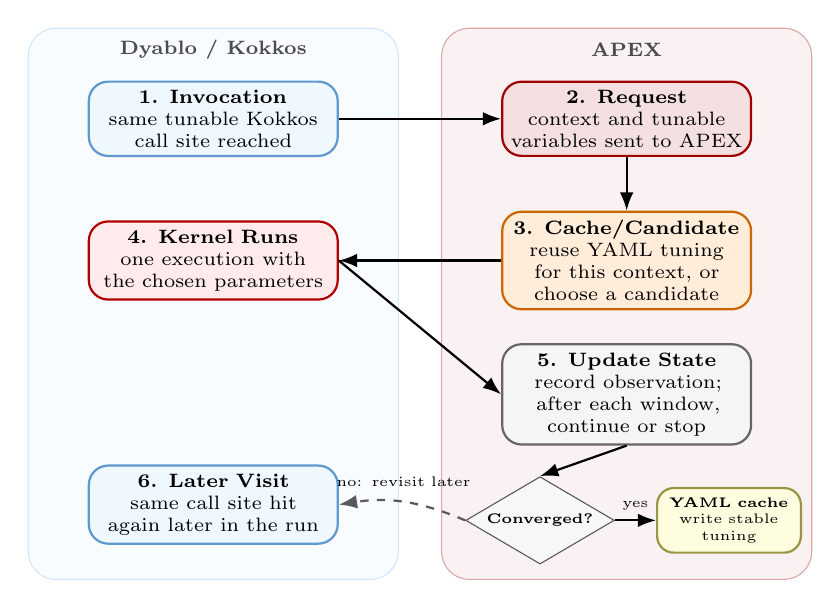
\begin{tikzpicture}[
  x=1cm,
  y=1cm,
  >=Latex,
  every node/.style={align=center},
  lane/.style={draw, rounded corners=10pt, minimum width=4.7cm, minimum height=7.0cm},
  lanehdr/.style={font=\scriptsize\bfseries, text=black!70},
  stage/.style={draw, rounded corners=7pt, thick, fill=white, minimum height=0.82cm, text width=2.95cm, inner sep=3pt, font=\scriptsize},
  decision/.style={diamond, draw=black!65, fill=black!3, aspect=1.7, inner sep=1.4pt, font=\tiny\bfseries},
  cachebox/.style={draw, rounded corners=6pt, thick, fill=yellow!12, draw=yellow!55!black, minimum height=0.82cm, text width=1.65cm, inner sep=2.5pt, font=\tiny},
  arr/.style={-Latex, thick},
  looparr/.style={-Latex, thick, dashed, draw=black!65}
]
\node[lane, fill=hotspotBlue!5, draw=hotspotBlue!35] at (1.85,-2.15) {};
\node[lane, fill=ceaGreen!5, draw=ceaGreen!35] at (7.1,-2.15) {};
\node[lanehdr] at (1.85,1.08) {Dyablo / Kokkos};
\node[lanehdr] at (7.1,1.08) {APEX};

\node[stage, fill=hotspotBlue!12, draw=hotspotBlue!80!black] (dy1) at (1.85,0.2)
  {\textbf{1. Invocation}\\same tunable Kokkos call site reached};
\node[stage, fill=ceaGreen!12, draw=ceaGreen] (ap1) at (7.1,0.2)
  {\textbf{2. Request}\\context and tunable variables sent to APEX};
\node[stage, fill=orange!15, draw=orange!80!black] (ap2) at (7.1,-1.6)
  {\textbf{3. Cache/Candidate}\\reuse YAML tuning for this context, or choose a candidate};
\node[stage, fill=red!8, draw=red!70!black] (dy2) at (1.85,-1.6)
  {\textbf{4. Kernel Runs}\\one execution with the chosen parameters};
\node[stage, fill=black!4, draw=black!60] (ap3) at (7.1,-3.3)
  {\textbf{5. Update State}\\record observation; after each window, continue or stop};
\node[stage, fill=hotspotBlue!12, draw=hotspotBlue!80!black] (dy3) at (1.85,-4.7)
  {\textbf{6. Later Visit}\\same call site hit again later in the run};
\node[decision] (conv) at (6.00,-4.9) {Converged?};
\node[cachebox] (yaml) at (8.4,-4.9)
  {\textbf{YAML cache}\\write stable tuning};

\draw[arr] (dy1.east) -- (ap1.west);
\draw[arr] (ap1) -- (ap2);
\draw[arr] (ap2.west) -- (dy2.east);
\draw[arr] (dy2.east) -- (ap3.west);
\draw[arr] (ap3.south) -- (conv.north);
\draw[arr] (conv.east) -- node[above,font=\tiny] {yes} (yaml.west);
\draw[looparr] (conv.west) to[bend right=16] node[below,font=\tiny,text width=1.9cm,xshift=-0cm,yshift=0.45cm]
  {no: revisit later} (dy3.east);
\end{tikzpicture}
\end{adjustbox}

\vspace{0.05em}
{\tiny\color{black!75}\textbf{Convergence:} once APEX stops searching for one context, it reuses that stable configuration and can write it to the YAML cache.}

\column{0.35\textwidth}
\begin{beamerboxesrounded}[upper=tuner title,lower=tuner body,width=\linewidth,shadow=false]{Context}
\tiny
\raggedright
A context is one tunable Kokkos call site.

\vspace{0.08em}
Here it is identified by \texttt{kernel name}, \texttt{kernel type}, and \texttt{tree node}.
\end{beamerboxesrounded}

\vspace{0.28em}
\begin{beamerboxesrounded}[upper=profiler title,lower=profiler body,width=\linewidth,shadow=false]{Tuned Knobs}
\tiny
\raggedright
\texttt{team\_size}, \texttt{vector\_length}, \texttt{tile\_0}, \texttt{tile\_1}, \texttt{tile\_2}
\end{beamerboxesrounded}

\vspace{0.18em}
\begin{beamerboxesrounded}[upper=terminal title,lower=terminal body,width=\linewidth,shadow=false]{Window / Cache}
\tiny
\raggedright
\texttt{window = 5}\\
update the candidate after 5 observations

\vspace{0.05em}
\texttt{Converged = true}\\
reuse later in the run and across runs

\vspace{0.05em}
\texttt{Converged = false}\\
later Dyablo runs may revisit the same APEX configuration search space, and the search may never converge
\end{beamerboxesrounded}
\end{columns}
\end{frame}

% =========================================================
\section*{Conclusion}
% =========================================================

\begin{frame}[fragile]
  \begin{center}
    \LARGE Thank you!\\[0.8em]
  \end{center}
  \begin{beamerboxesrounded}[upper=terminal title,lower=terminal body,width=0.82\linewidth,shadow=false]{%
  \textcolor{red!70}{\footnotesize\textbullet}\hspace{0.15em}%
  \textcolor{yellow!80}{\footnotesize\textbullet}\hspace{0.15em}%
  \textcolor{green!70!black}{\footnotesize\textbullet}\hspace{0.55em}%
  \texttt{\scriptsize APEX}}
{\footnotesize\color{termText}
{\color{red!80!white}\verb!          (            )!}\\
{\color{hlOrange}\verb!   (      )\ )      ( /(!}\\
{\color{hlOrange}\verb!   )\    (()/( (    )\())!}\\
{\color{red!80!white}\verb!((((_)(   /!}{\color{yellow!80}\verb!(_)!}{\color{hlOrange}\verb!)))\  (!}{\color{yellow!80}\verb!(_)!}{\color{red!80!white}\verb!)\!}\\
{\color{red!80!white}\verb! )\ _ )\ !}{\color{yellow!80}\verb!(_)!}{\color{hlOrange}\verb!)) (!}{\color{yellow!80}\verb!(_)!}{\color{hlOrange}\verb!) !}\verb!__!{\color{hlOrange}\verb!(!}{\color{yellow!80}\verb!(_)!}{\color{red!80!white}\verb!)!}\\
{\color{red!80!white}\verb! !}{\color{yellow!80}\verb!(_)!}\verb!_\!{\color{yellow!80}\verb!(_)!}\verb!| _ \| __|\ \/ /!\\
\verb!  / _ \  |  _/| _|  >  <!\\
\verb! /_/ \_\ |_|  |___|/_/\_\!
}
  \end{beamerboxesrounded}
  \begin{center}
    \normalsize \email
  \end{center}
\end{frame}

\end{document}
